\documentclass{book}

\usepackage{listings}
\usepackage{theorem}
\usepackage{graphicx}
\usepackage{hyperref}
\usepackage{amsfonts}
\usepackage{amsmath}
\usepackage[table]{xcolor}
\usepackage{array,calc}
\usepackage{amsmath}

\newtheorem{exercise}{Exercise}


\lstset{
  language=Java,
  basicstyle=\ttfamily\footnotesize,
  numbers = left
}

\newcommand{\co}[1]{\lstinline[language=Java, basicstyle=\ttfamily]{#1}}

\begin{document}

\addtocounter{chapter}{3}

\chapter{Point Operations}
A point operation is an image processing step that takes an image as input and that outputs a new image by applying a function to the color of each pixel in the input image. That is, the color of each pixel in the output image depends only on the color of the corresponding pixel in the input image. More formally, each point operation has a corresponding function $f$ that maps colors to colors. The point operation itself applies this function to each pixel:
$$I'(x, y) \leftarrow f(I(x, y))$$
for each position $(x, y)$ in the image. For example, inverting a grayscale image is a point operation with function $f(c) = 255 - c$. Similarly, the identify transform is a point operation with function $f(c) = c$. As we will explain in Section~\ref{sec:contrast-stretching}, the function being applied can depend on the image itself.

In the remainder of this chapter, we will study a number of point operations.

\section{A Tiny Framework for Point Operations}
Each point operation applies a function to each pixel in the image. To model the common aspects shared by all point operations, we define an abstract class \co{PointOperation}. 
\begin{lstlisting}
public abstract class PointOperation {
  public abstract int f(int color);
  
  public void applyTo(ImageProcessor ip) {
    for(int x = 0; x< ip.getWidth(); x++) {
      for(int y = 0; y < ip.getHeight(); y++) {
        ip.putPixel(f(ip.getPixel()));      
      }    
    }
  }
}
\end{lstlisting}
Specific point operations will be modelled by subclasses of \co{PointOperation}. In particular, subclasses should override the abstract method \co{f} with their own function. The method \co{applyTo} modifies the given \co{ImageProcessor} by applying \co{f} to each pixel. Let's look at an example. Inverting a grayscale image is a point operation with function $f(c) = 255 - c$. We can represent inversion by defining a subclass of \co{PointOperation} that overrides \co{f}. 
\begin{lstlisting}
public class Gray8Invert extends PointOperation {
  @Override  
  public int f(int color) {
    return 255 - color;
  }
}
\end{lstlisting}
A grayscale image can be inverted as follows:
\begin{lstlisting}
ImageProcessor ip = ...
Gray8Invert invertor = new Gray8Invert();
invertor.applyTo(ip);
\end{lstlisting}
We can visualize the function corresponding to a point operation in a plot. For example, the plot corresponding to grayscale inversion is the following:
\begin{center}
\includegraphics[scale=0.15]{inversion-plot.png} % todo: better plot
\end{center}

\begin{exercise}
Thresholding is a point operation that converts a grayscale image to a binary image by mapping dark pixels to black and light pixels to white. The function for thresholding is the following:
$$threshold(c) = \left\{\begin{array}{c l}
  0 & \text{if $c \leq 127$}\\
  1 & \text{otherwise}\\
\end{array}
\right.$$
Draw the plot corresponding to thresholding and implement thresholding by defining a new subclass \co{Gray8Threshold} of \co{PointOperation}. Thresholding \co{lena-gray.png} results in the following image:
\begin{center}
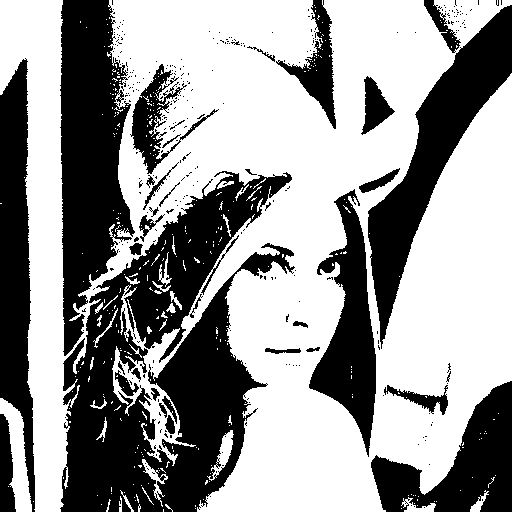
\includegraphics[scale=0.10]{lena-binary.png}
\end{center}
\end{exercise}

\begin{exercise}
Modify \co{Gray8Threshold} such that the bound (\co{127}) is no longer fixed. More specifically, add a constructor that takes the bound as an argument. Thresholding \co{lena-gray.png} with bound 180 results in the following image:
\begin{center}
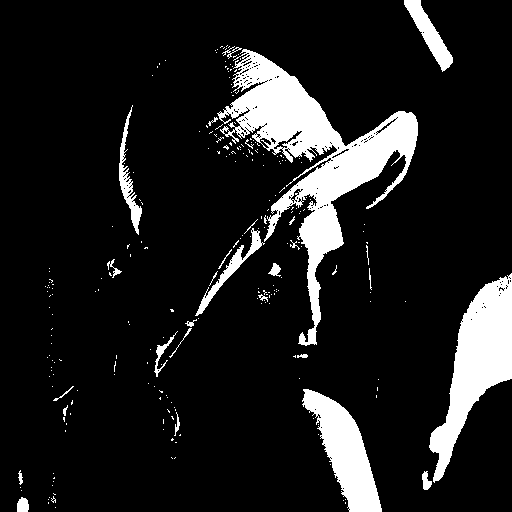
\includegraphics[scale=0.10]{lena-binary-bound-180.png}
\end{center}
\end{exercise}

\begin{exercise}
Thresholding reduces the number of colors in the image to two, black and white. Posterization is a generalization of thresholding to multiple colors. For example, when posterizing a grayscale image to three colors, the range 0 to 85 is mapped to 0, 86 to 170 is mapped to 128 and finally colors in the  range 171 to 255 are mapped to 255. Thus, the function for 3-color posterization is the folllowing:
 $$posterize3(c) = \left\{\begin{array}{c l}
  0 & \text{if $0 \leq c \leq 85$}\\
  128 & \text{if $86 \leq c \leq 170$}\\
  255 & \text{if $171 \leq c \leq 255$}\\
\end{array}
\right.$$
The plot corresponding to this function looks as follows:
\begin{center}
%\includegraphics[scale=0.10]{posterize3-plot.png} % todo
\end{center}
Implement a point operation \co{Gray8Posterize} to posterize grayscale images. The desired number of colors should be a parameter of the class' constructor. Posterizing \co{lena-gray.png} to 4 colors results in the following image:
\begin{center}
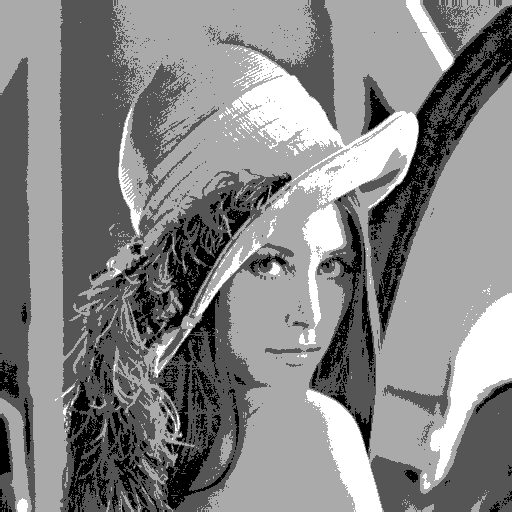
\includegraphics[scale=0.20]{lena-gray-posterized4.png}
\end{center}
\end{exercise}

\begin{exercise}
Implement a point operation \co{ConvertToSepia} that converts an RGB color image to sepia. The function corresponding to sepia conversion maps an RGB triple to a new RGB triple. This function is not standardized, but we will use the following definition:
$$\begin{array}{c}
sepia((r, g, b)) = \\
({gray}+ 2.{sepiaDepth}, {gray} + {sepiadepth}, {gray} - {sepiaIntensity})\\
\end{array}$$
where $gray = (r + g + b) / 3$ and ${sepiaDepth}$ and ${sepiaIntensity}$ are parameters of the conversion. This function increases the values of the red and green channel to make the image more yellow.  Setting ${sepiaDepth}$ to $20$  and ${sepiaIntensity}$ to $30$ produces nice result. The following image was generated from \texttt{lena.png} based on these parameters:
\begin{center}
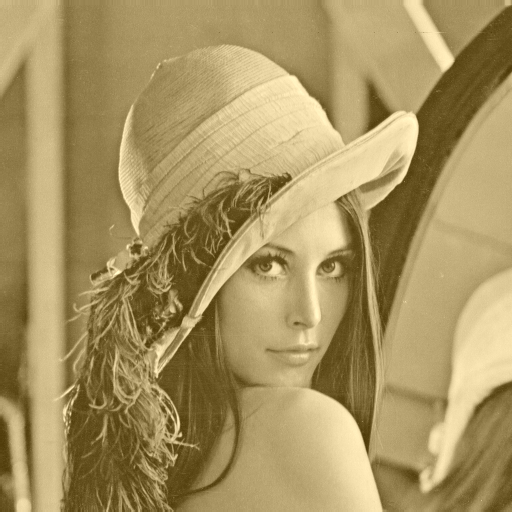
\includegraphics[scale=0.20]{lena-sepia.png}
\end{center}
\end{exercise}

\section{Grayscale Contrast Stretching}\label{sec:contrast-stretching}
The contrast of a grayscale image is the difference between the minimum and maximum pixel value used by the image. An image with low contrast can appear to be dull and not lively colors. For example,
the images shown below have decreasing contrast (from left to right).
\begin{center}
%todo
\end{center}
Contrast stretching is a point operation that stretches the contrast of an image to the entire available range. The idea is to pull the entire histogram to the left and then stretch it until the maximum falls on 255 as shown below.
\begin{center}
%todo
 \end{center}

\subsection*{Improved Grayscale Contrast stretching}

\section{Multi Image Point Operations}

\subsection{Alpha-blending}

\subsection{Chroma Key Compositing}

\section{Color Contrast Stretching}\label{sec:color-contrast-stretching}

%\section{Post-it Images}

\end{document}